\chapter{Framework: Pipes and Filters}
\label{newframework}

In this chapter, we design a framework based on the theoretical model from previous chapter. We start by establishing a small and general core architecture and continue with how we extended and used this core to build a flexible author-disambiguation tool. Implementation details of the framework and used algorithms and technologies in this framework will be discussed as well. Throughout the design, the requirements set in the foundation \autoref{foundation} and theoretical model were taken into account. At the end of the chapter we will discuss the strengts and weaknesses of the framework.

% aspect, flow, identifier, enrich, filter

\section{Small and Simple Core}

We opted for a small and simple core framework. It is based on Pipes and Filters with a few extension. We chose to use this design pattern for the following reasons:

\begin{enumerate}
\item \textbf{Scalability} As said in Foundation \autoref{foundation:endless}, our algorithm needs to scale. Pipes and Filters makes this easy as all component are treated equally, can run independent from others and have a common interface.
\item \textbf{Modifiability} The Foundation (\autoref{foundation}) points to the highly dynamic environment several times. The framework will thus constantly be subject to new developments. These new developments will be in the form of new pipes, which can be plugged into the framework at any place.
\item \textbf{Maintainability} Using Pipes and Filters will reduce the complexity added by constantly modifying the framework. Pipes can always simply be replaced, moved and reconfigured in any way.
\end{enumerate}

\subsection{Architecture}

In figure \autoref{fig:architecturev2}, the architecture for the small Pipes and Filters core is shown. Each pipe has a number of input and output connectors. These connectors can be coupled to connectors of other pipes with a connection. When a pipe has executed it pushed its processed flow into the appropriate connector. This connector then pushes it to the connection that again pushes the flow into the connector of the next pipe. This pipe is then executed on the flow.

\begin{figure}[htp]
	\centering
		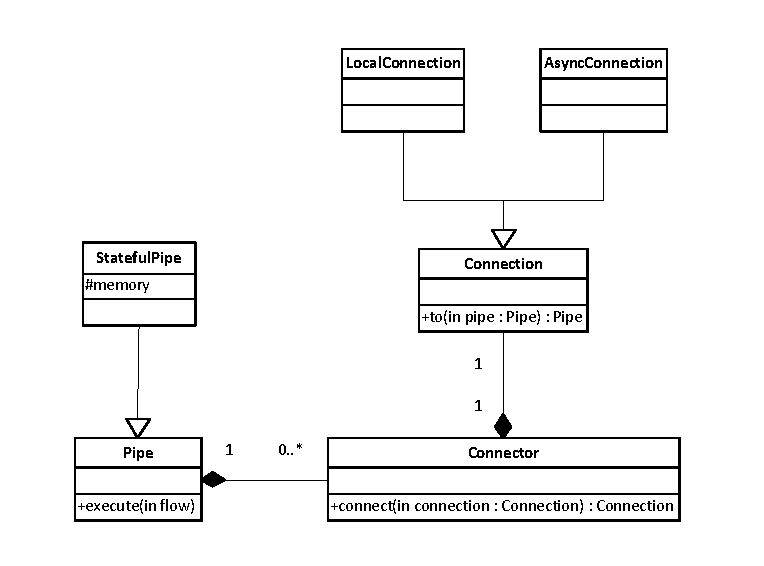
\includegraphics[width=0.8\textwidth]{fig/architecturev2}
	\caption{Pipes and Filters based Architecture.}
	\label{fig:architecturev2}
\end{figure}

The three classes Pipe, Connector and Connection are the real core of the architecture. All extensions and software to be created using this core will probably extend Pipe or Connection. Three important extensions are already present in the core architecture: LocalConnection, AsynConnection and StatefulPipe. These classes will be discussed later on.

\subsection{Concepts, Terminology and Notations}

Together with this architecture we developed a few concepts that we use in combination with the core framework. These concepts allow us to build pipe configurations more easily and give us flexible control over the data flowing to the system. These concepts and associated terminology are explained in the following paragraphs.

\paragraph{Flows and Aspects} The information flowing through the pipes and connections are flows. Flows exist of different aspects. Every pipe is only interested in a few aspects of a flow. Other aspects can travel along too feed pipes later on the path. The choice of which aspect we process or send is completely free. An example of aspects are instance, publication or dependencies (see ... REF).

\paragraph{Connector Identifiers} Connectors need to be identified to allow us to connect a specific input or output to the right connection. The identifiers of the connectors can be any object. This makes configuring the pipes more expressive as identifiers suiting the context of the pipe can be used. For example, the output connector identifiers of the Filter pipe (\autoref{par:filterpipe}) are the booleans "true" and "false". We denote a input-connector with identifier $x$ as $Cn^i_x$ and an output-connector with identifier $y$ as $Cn^o_y$. The output ports of the Filter pipe would thus be denoted as $Cn^o_{true}$ and $Cn^o_{false}$.

\paragraph{Flow enrichment and filtering} In every pipe, we can push out whatever we want. However, a much used situation is where the pipe outputs the input flow with an extra aspect or a modified aspect. We call this flow enrichment. The other way around is also a possibility, any aspect or part of an aspect can be filtered in any pipe. However, this is not used in regular pipes but in a dedicated Filter pipe (\autoref{par:filterpipe}). Enriching and Filtering are denoted with plus and minus signs on the flow. An enriched flow A can be indicated with $A^+$ and a filtered flow A with $A^-$. The aspect that has been filtered or added can be indicated between brackets.

\paragraph{Flow Rate} Some pipes can increase or decrease the flow rate. A Filter for example will decrease the flow rate on both output connections. A Rule on the other hand will probably output multiple similarities for one input. Increasing the flow rate is denoted by adding a star (*) to the flow notation at the output. Decreasing the rate is indicated by a star on an input flow.

The notations we introduced are summarized in \autoref{fig:pipecomponents}.

\begin{figure}[htb]
	\centering
		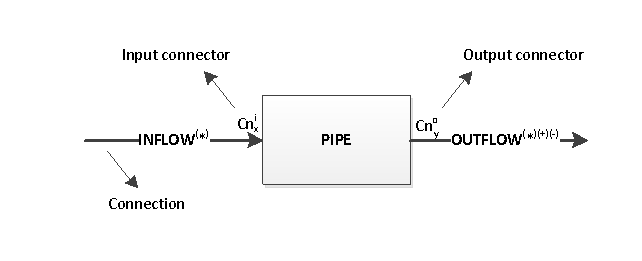
\includegraphics[width=0.75\textwidth]{fig/pipecomponents}
	\caption{Pipe components, terminology and notations.}
	\label{fig:pipecomponents}
\end{figure}

\subsection{Core Extensions}

In the architecture (\autoref{fig:architecturev2}), we already mentioned three core extensions. These extensions extensively used throughout the program, so we included them in the architecture. Each of these three extensions is explained below.

\paragraph{Local Connections}

The most basic connection between two local pipes is one that just pushes the flow forward without memorizing anything. This connection is the bread and butter of configuring pipe networks in our program.

\paragraph{Asynchronous Connections}

A more complex connection is the asynchronous connection. It allows us to run any pipe in a distributed way. When a connection is made asynchronous, the flow of the pipe will be interpreted as the description of a job. This job will be pushed to a queue in a distributed shared memory store. A predefined set of workers ran on different machines will poll this queue constantly and execute the jobs on the machine they are running. This way, the load pushed to the pipes can be evenly distributed over a set of nodes in a computing cluster. The technology we use for this and extra details can be found in \autoref{resque}.

\paragraph{Stateful Pipes}

For some pipes, it is required to have a non-transient memory, a memory that survives between executions. This allows the pipe to process input differently based on what is present in its long-time memory. As Pipes can be run in a distributed fashion, it is possible for a pipe to be initialized on another physical machine for every execution. If the memory would be local, bound to a machine, the pipe would lose access to it if it was executed on another machine. To solve this, we use a distributed shared memory store (\autoref{redis}.

\subsection{Implementation details and Technologies}

\paragraph{The Use of Ruby and Java}

\paragraph{A Distrbuted Shared Key-Value Store: Redis}

\paragraph{A Distributed Job Processing Framework: Resque}

\section{Generally Useful Pipes}

With these small and simple Pipes and Filters core we built some useful pipes along the way. Clearly the filter pipe is important to have in a Pipes and Filters architecture, so we explain this one first. Merging and Splitting flows, both extensively used pipes, are mentioned second. Thirdly we introduce a pipe that allows us to do network operations. Last, we discuss two pipes more specific for our case but as yhey are used troughout the entire pipe system, we mention them here.

\paragraph{Filter} \label{par:filterpipe} The Filter pipe allows us to filter flow in two ways, as you can also see on \autoref{fig:filter}. First, it is possible to test a condition for each arriving flow. Depending on this condition, the flow is forwarded to either the connector with identifier "true" or identifier "false". On top of that we are able to filter aspects of the flow itself. This Filter pipe gives us the possibility to control the flow in our pipe configuration. The flows should be small and contain only aspects that are necessary.

\begin{figure}[htp]
	\centering
		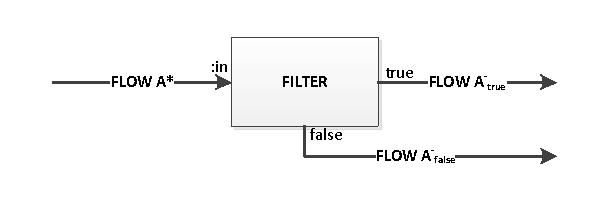
\includegraphics[width=0.75\textwidth]{fig/filter}
	\caption{Filter pipe.}
	\label{fig:filter}
\end{figure}

\paragraph{Merge and Split} In the case we want to forward the result from one pipe to multiple pipes or from multiple pipes to one, we need a Split or Merge pipe. Split pipes have the default ":in" connector and split their input over $n$ output connectors identified by $1,\ldots,n$. A Merge pipe does the inverse by merging input connections $1,\ldots,n$ into one connector identified by the default ":out".

\begin{figure}[htb]
	\centering
		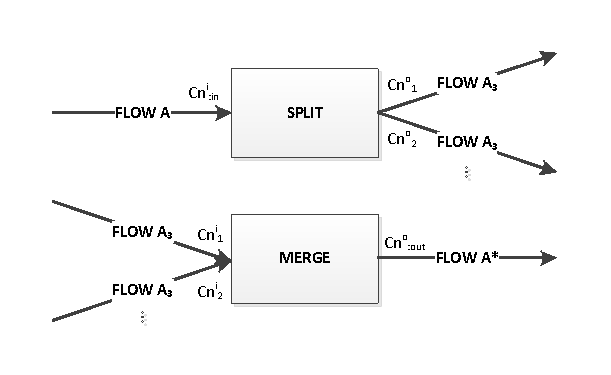
\includegraphics[width=0.75\textwidth]{fig/mergeandsplit}
	\caption{Merge and Split pipes.}
	\label{fig:mergeandsplit}
\end{figure}

\paragraph{Network}

\section{Working Towards a Contextual System}

We now apply these general concepts and designs in the context of our thesis problem. First we agree upon a set of flow types. A flow type marks a flow and is used to distinguish flow from each other. In short, the path of a flow through a pipe configuration will depend on its type.

\subsection{Flow Types} We divide flow into four types. Two of these types carry crawled information from the web. The flow associated with these types are "information flows. The other two accompany "control messages". We indicate the type of flow $A$ as $A_type$.

\begin{enumerate}
\item \textbf{Discovery}: The discovery of a new piece of information. The source can be anything but will be probably the web or a publication document. The most important discoveries are instances and publications.
\item \textbf{Fact}: The finding of a relation between two entities is called a fact. The most important flow with this type the one with the fact that a certain instance published a publication.
\item \textbf{Similarity} Rules (\autoref{rules}) process these two types and generate similarities. These similarities are again sent through as a flow message.
\item \textbf{Cluster} Similarity messages are intended for clustering pipes, these pipes interpret the similarities and make the appropriate changes in the author clusters.
\end{enumerate}

After establishing these four main message types, we created another two generally usable pipes both further explained below.

\paragraph{Persist Discovery}

\paragraph{Persist Fact}

\subsection{Implementation details and Technologies}

\paragraph{A Graph Database: Neo4j in Combination With the Tinkerpop Stack}

\section{Helper Modules}

\subsection{Locking}

\section{Pipe Configuration}

In this section we will give an overview of the entire pipe configuration of our program. We have devided this configuration into parts, each with their own responsibilities, difficulties and used technologies. We first discuss the parts that form the structural layer, followed by the informational layer and the similarity layer.

\subsection{Instance Integration}

When a new instance is discovered, it has to be integrated in the graph. Later on, information can be attached to this instance to feed the rules. The different steps of this integration have been explained in \autoref{structurallayer}. An overview of the pipe configuration is found in \autoref{fig:integrationpipe}.

First, the incoming instance discovery is lead to the "Persist Instance" pipe. This pipe persists the instance in the graph. As every new instance is assigned its very own author (cluster), the cluster is also persisted and the appropriate edges are added. The subsequent two pipes on the path deal with the persisting the family and the name nodes. If a name is already present in the system, the integration of the instance has finished. Otherwise, we must execute a name matching algorithm. This algorithm is explained in the next paragraph.

\begin{figure}[htb]
	\centering
		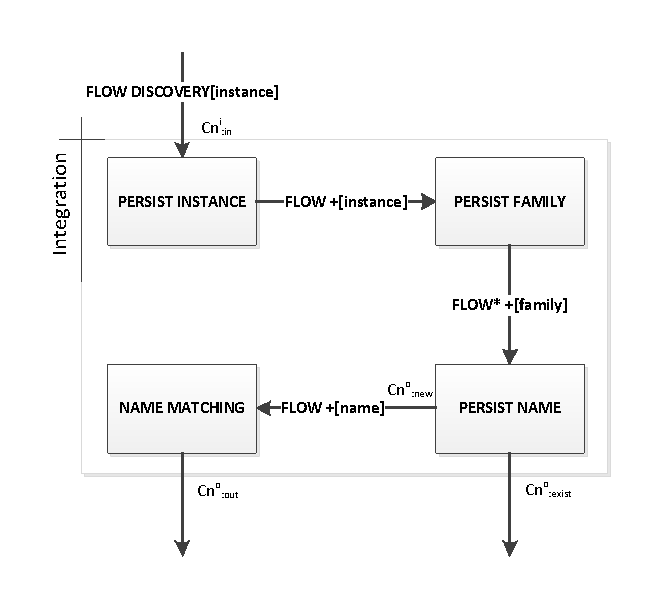
\includegraphics[width=0.75\textwidth]{fig/integrationpipe}
	\caption{Pipe Configuration for Instance Integration.}
	\label{fig:integrationpipe}
\end{figure}

\paragraph{Name Matching} Name Matching is the process of matching the name of a family with the names already present in the family. The goal is to reduce the problem domain size (\autoref{problemdomain}. When a new name is added, we query all the names in the family and compare them to the name that is being added. We do this using a fuzzy string matching algorithm based on Dynamic Time Warping. Taking properties of names into account lead to some modifications of the algorithm, making it especially suitable for name matching.

\begin{enumerate}
\item We use a token based approach (tokens between whitespace). The tokens themselves are compared using the Jaro Winkler fuzzy string matching algorithm.
\item The algorithm is always started from the viewpoint of the name with the least amount of tokens. An insertion has a cost of zero and a deletion is heavily penalized.
\item In case of a short token (one symbol or one symbol followed by a dot), we do not use a fuzzy approach. If the first letter matches with the first letter of the token it is being compared with, we assign a minimum cost, otherwise we assign a maximum cost.
\end{enumerate}

\subsection{Magic Facts}

As we also make use of email and affiliation rules, we needed to find a way to collect this data. We first attempted to retreive publication documentes via Microsoft Bing. Google scholar is not usable due to its security against programmatic access. The number of publications found by Bing was not enough to feed the rules. Although we created a pipe that can extract email addresses out of PDF documents and assign them to the correct author, we did not use it. We did this partly because information retrieval is not our main focus and not the real challenge. It is definitely possible to collect all this data with more effort. However, we thought it was more important to research the power of this information in the context of disambiguation.

To still be able to use the data, we manually collected email addresses and affiliations out of the publications of the authors in our testset. As this information makes a magical appearance in our system, we called the pipe that provides it "Magic Facts".

\subsection{Publications}

\begin{figure}[htb]
	\centering
		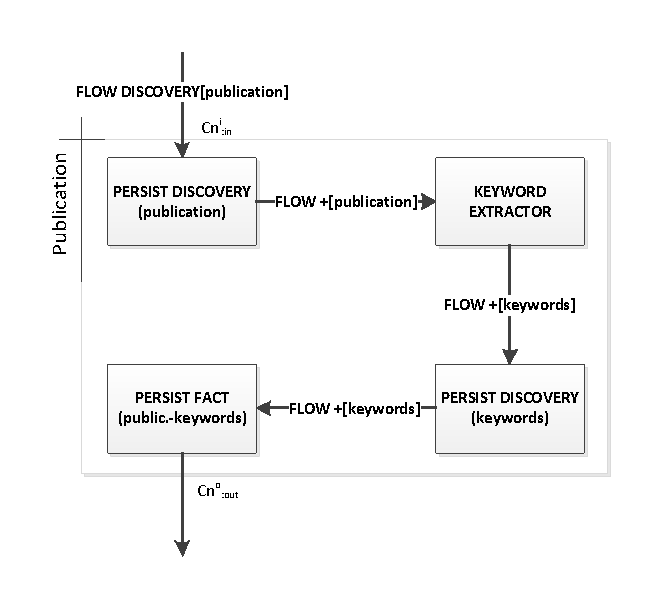
\includegraphics[width=0.75\textwidth]{fig/publicationpipe}
	\caption{Pipe Configuration for Publication Processing.}
	\label{fig:publicationpipe}
\end{figure}

\subsection{Rules}

\subsubsection{Community Rule}

\subsubsection{Interest Rule}

\subsubsection{Email Rule}

\subsubsection{Affiliation Rule}

\section{Inside the Pipes}

\subsection{Dependency Resolution}

\subsection{Concurrent, incremental Clustering}

Clustering is a very important step in building towards a solution. Each new flow of information indirectly leads to a clustering operation. Acquiring new information triggers rules which on their turn yield similarities. These similarities change the balance between clusters. In the worst case, an expensive rebalancing procedure is necessary.

It is obvious that processing similarities is something that will be executed very frequently (numbers?). The combination of the enormous amount of similarities and their expensive processing requires us to make this process as streamlined and efficient as possible. The clustering algorithm as explained in [REF] leads to a first, na\"ive implementation approach. Rethinking the absolute needs of the clustering algorithm then leads to a second approach that benifits greatly of the foundations of our framework.

\paragraph{In-graph implementation} The most simple solution one can think of is to maintain the ICW and OCW for every vertex in the vertex itself. The adjacency matrix would implicitly be defined by the edges between two nodes in the similarity plane. This technique has two main drawbacks:

\begin{enumerate}
\item A lot of load would be pushed to the database.
\item There would be a need for several concurrency control mechanisms/
\end{enumerate}

If clustering could be executed without the use of the database in an efficient manner, it would be preferrable. After all it is in our best interest to take as much load as possible away from the database because it is much more difficult to scale than our pipes and filters architecture. Besides, the similarity ``meta''-plane is not something that should be queried from our end-user application. The users are interested in the result of the clustering, not the way it got there.

In the case of similarities being processed in parallel, we need to pay some extra attention. We do not want that the clustering mechanism inflicts race conditions and, by consequence, inconsistencies on the graph.


\paragraph{As a stateful pipe}

\begin{algorithm}
\caption{!!!}
\label{mincutgusfield}
\begin{algorithmic}
\STATE \textbf{lock} $I_1,I_2$
\IF{cluster($I_1$) == cluster($I_2$)}
  \STATE \textbf{watch} $C_1,C_2$
  \STATE \textbf{unlock} $I_1,I_2$
  \STATE \textbf{process(intra-cluster)}
\ELSE
  \STATE \textbf{lock} $C_1,C_2$
  \STATE \textbf{unlock} $I_1,I_2$
  \STATE \textbf{process(inter-cluster)}
  \STATE \textbf{execute}
  \STATE \textbf{unlock} $C_1,C_2$
\ENDIF
\end{algorithmic}
\end{algorithm}

\begin{figure}[htb]
	\centering
		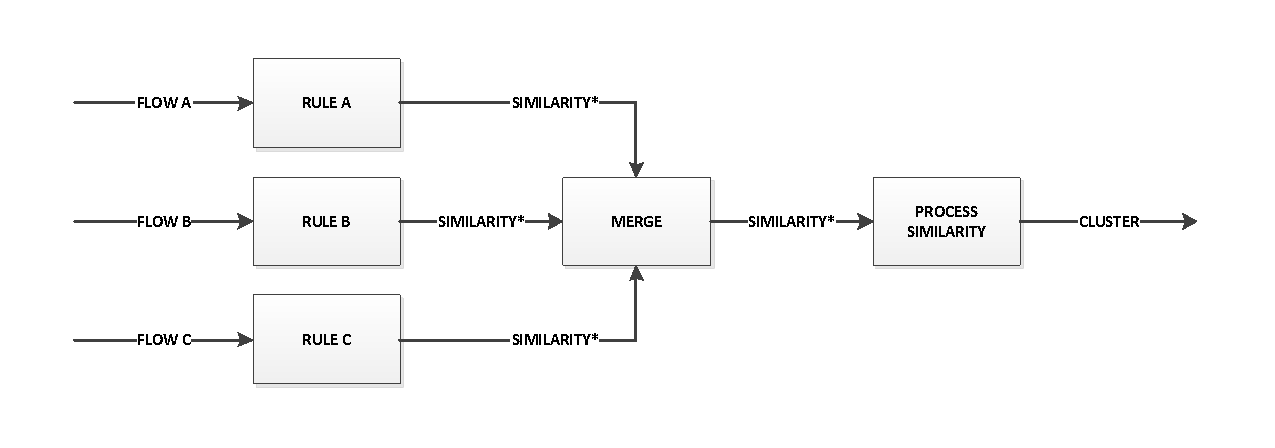
\includegraphics[width=1\textwidth]{fig/clusteringpipe}
	\caption{Clustering flow}
	\label{fig:clusteringpipe}
\end{figure}

\subsection{Assignment of e-mail addresses}